
%%%%%%%%%%%%%%%%%%%%%%%%%%%%%%%%%%%%%%%%%%%%%%%%%%%%%%%%%%%%%%%%%%%%%%%%%
%           Capítulo 2: MARCO TEÓRICO - REVISIÓN DE LITERATURA
%%%%%%%%%%%%%%%%%%%%%%%%%%%%%%%%%%%%%%%%%%%%%%%%%%%%%%%%%%%%%%%%%%%%%%%%%

\chapter{La Asimetría Bariónica y el Experimento AMS-02}
\section{Nucleosíntesis del Big Bang}


\section{Rayos cósmicos}

\begin{figure}[h!]
    \centering
    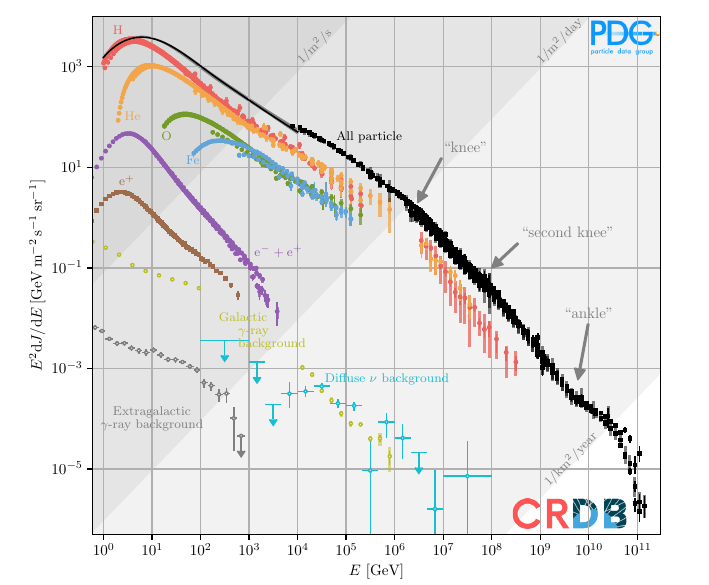
\includegraphics[scale=0.6]{Tesis-UNAM/Capitulo2/RCespectro.png}
    \caption{Espectro de los RC's}
    \label{fig:enter-label}
\end{figure}
Los Rayos Cósmicos(RC) son un conjunto de partículas no termales que permean el universo, una forma de caracterizar los RC es a través de su espectro, composición y su distribución espacial. Para RC cargados, por ejemplo, su espectro se extiende desde unas decenas de MeV's a casi 1 ZeV. La distribución espectral obedece diferentes leyes de potencias i.e. $E^{-\gamma}$\cite{Workman:2022ynf}. Dependiendo del rango de energía el factor $\gamma$ cambia, lo que da a lugar a decir que presenta varias estructuras. Para energías menores a unos cuantos PeV, el indice espectral $\gamma \approx 2.7$, a mayores energías el indice cambia a ~3, esta estructura se le llama la rodilla, para energías encontramos la segunda rodilla, donde $\gamma \approx3.3$ y por último los RC más energéticos que 1 EeV $\gamma \approx2.5$ forman una estructura denominada "tobillo"\cite{Workman:2022ynf}.\\

La composición de los RC consiste mayormente en protones, helio y demás nucleos, aun que también se encuentran positrones, electrones, antiprotones, y recientemente el experimento AMS ha detectado antinucleos\cite{Doetinchem_2020}. La distribución espacial es mayormente isotrópica, aun que debido al campo magnético galáctico y la disposición de las fuentes se han observado anisotropias alrededor de la "rodilla"\cite{Workman:2022ynf}; además de los RC cargados, rayos gamma y neutrinos altamente energéticos también componen parte de los RC.\\

Los RC cargados son desviados numerosas ocasiones por varios campos magnéticos, así que la dirección en la que son detectados no apunta hacía su fuente\cite{Workman:2022ynf}. Dependiendo de la energía se piensa que los RC son galácticos ($<$PeV) y extragalácticos ($>$EeV).\cite{Workman:2022ynf}\\

Algunos posibles candidatos a fuentes se asocian principalmente a las últimas etapas de la vida estelar, o a agujeros negros supermasivos que emiten gran cantidad de energía rotacional y gravitatoria\cite{Workman:2022ynf}. Se ha pensado como posibles fuentes galácticas a microcuásares, el centro de la via láctea, o viento estelar de clusteres de estrellas, mientras que para las extragalácticas se piensa que son núcleos galácticos activos, pulsares, magnetares y galaxias con brotes estelares\cite{Workman:2022ynf}.\\

\begin{figure}
    \centering
    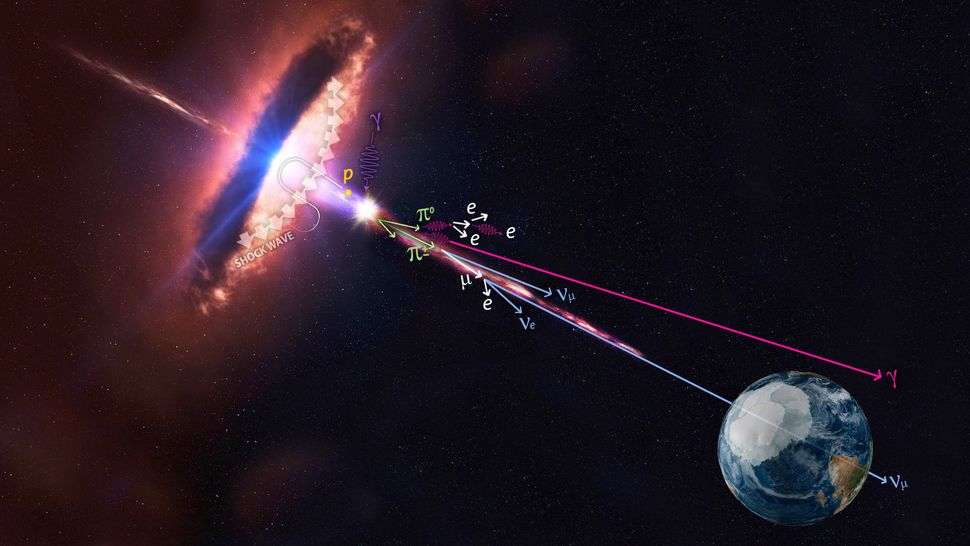
\includegraphics{Tesis-UNAM/Capitulo2/cosmicRays.jpg}
    \caption{Diagrama Ilustrativo de Los Rayos Cósmicos y sus Fuentes}
    \label{fig:enter-label}
\end{figure}

Dentro de la Vía Láctea, el proceso de transporte más importante de los rayos cósmicos es la difusión\cite{Workman:2022ynf}, cómo lo demuestran las anisotropías en las direcciónes de llegada y mayor abundancia de algunas especies nucleares, este mecanismo difusivo se debe a las múltiples interacciones de los RC cargados con los campos magnéticos presentes en el Universo. Aun que también otros procesos contribuyen al transporte observado, cómo son, perdidas de momento, perdidas radiativas, ionización, espalación (creación de nucleos más ligeros a partir de colisiones inelásticas)\cite{Workman:2022ynf}. \\

El estudio de los rayos cósmicos puede ser provechoso para la comprensión de fenómenos astrofísicos, ya que constituyen una parte muy considerable del contenido energético en varios ambientes en el Universo. La presión de los RC es tal que pueden modificar su entorno, e.g. Los RC contribuyen a la estructura gravitacional de las galaxias, y pueden impulsar flujos de salida en escalas galácticas. También los rayos cósmicos causan turbulencias lo que afecta en gran medida el transporte galáctico y la aceleración de choque\\

La física fundamental también se beneficia notablemente del estudio de RC, por ejemplo si la materia oscura(MO) interacciona con el modelo estandar, uno podría observar productos de auto-aniquilaciones o de decaimientos de la MO. Otro gran enigma que podrían elucidar los RC es sobre la asimetría matera-antimateria, dado que por mucho la gran mayoria de rayos cósmicos son conformados de materia ordinaria. Por último ha habido un exceso de rayos-$\gamma$ y neutrinos detectados provenientes del núcleo de la Vía Lactea, lo cuál concordaría con las predicciones de algunos modelos de MO \cite{Workman:2022ynf}\\

% Incluir información sobre antinúcleos en rayos cósmicos
% Hablar sobre su producción secundaria por rayos cósmicos con el medio interestelar y también sobre la posible producción por materia oscura
% Los antinucleos detectados por AMS


\section{Radiación Cherenkov}
\subsection{Descubrimiento}
Pavel A. Cherenkov, en los años de 1930 a 1935 realizó su doctorado sobre la luminiscencia de soluciones de sales de uranilo bajo la acción de rayos-$\gamma$, Cherenkov investigó el fenómeno de la luminiscencia inducida por rayos-$\gamma$ de una fuente de radio comparandola con la emisión de luz luminofora.\cite{CHERENKOVA20088}\\
%\subsubsection{Técnicas Experimentales}
%Para todos estos estudios se utilizaron dos fuentes unicamente, rayos X y luz visible y dado que la intensidad de la luz fué mínima, se requería un diseño de un dispositivo de fotometría lo suficientemente sensible para poder realizar mediciones cuantitativas; Cherenkov se decidió por una cuña óptica con el ojo humano cómo detector óptico. \\

%El montaje experimental se describe en la figura 2.1, el recipiente A con el líquido luminóforo y la fuente radioactiva se posan sobre un soporte B, el espesor promedio del recipiente son tales que la radiación $\alpha$ y $\beta$ sea absorbida pero los rayos-$\gamma$ puedan atraversar el contenedor, el soporte B poseé dos ranuras $R_1$ y $N_2$ donde se colocaron pequeñas muesras de radio el prisma nicol $N$ se puede utilizar para realizar medidas sobre la polarización de la luz, también se utilizo un colimador $L_1$ un prisma P, un telescopio formado por dos lentes $L_1$ y $L_2$ y la cuña óptica K, varios filtros ópticos se pueden montar en el marco E, y el diafragma D define el campo de visión.
%A pesar de la simplesa del diseño experimental, Cherenkov pudo realizar las mediciones con una alta precisión.
%\begin{figure}[h!]
    %\centering
    %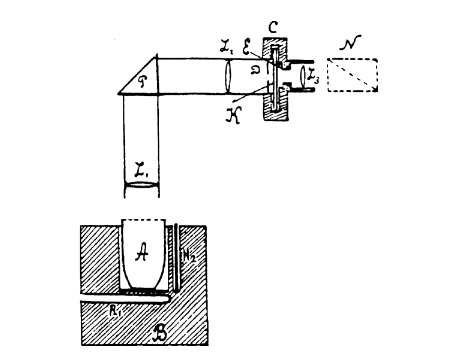
\includegraphics[scale=0.6]{Tesis-UNAM/Capitulo2/experimentoCerenkov.png}
    %\caption{Esquema del montaje experimental}
    %\label{fig:enter-label}
%\end{figure}
%\\\\%

Al realizar sus experimentos en luminiscencia, Cherenkov se dió cuenta de un fenómeno peculiar, al incidir rayos-$\gamma$ sobre ácido sulfúrico\cite{CHERENKOVA20088}, se presentaba una pequeña emisión de luz azul, hoy sabemos que esto fue radiación cherenkov emitida a causa de electrones acelerados por dispersión compton debida a los rayos-$\gamma$. También se estudió la polarización de esta radiación electromagnética\cite{Bashmakov_2015}, bajo condiciones óptimas se obtuvo un 20$\%$ de polarización total, donde el plano dominante del campo eléctrico era paralelo a la dirección de propagación de los rayos-$\gamma$. \\\\
En posteriores experimentos Cherenkov implementó una geometría axiosimétrica, un contenedor cilíndrico transparente con el líquido a estudiar, se rodeó de un espejo con una geometría cónica, subsecuentemente el recipiente se cubrió con una cubierta que no era transparente a la luz, y la fuente radioactiva se colocaba en el exterior del espejo\cite{Bashmakov_2015}. Gracias a estas investigaciones se descubrió una de las características más interesantes de esta emisión lumínica, la cuál la diferencían de las radiaciones previamente conocidas a los estudios de Cherenkov - su asimetría espacial\cite{Bashmakov_2015}. Este descurbrimiento le valió el Premio Nóbel de Física de 1958 a Cherenkov.

\subsection{Descripción y Naturaleza del Fenómeno}
La descripción teórica del fenómeno fue desarrollada por I.M. Frank e I.E. Tamm\cite{Bashmakov_2015, Jelley, CHERENKOVA20088}, la cual fue verificada posteriormente por P. Cherenkov. Donde hicieron una analogía con las ondas Mach de la hidrodinámica (Aunque Sommerfeld y Heaviside ya habian predicho la emisión de luz por partículas cargadas moviendose a velocidades supralumínicas previamente)\cite{CHERENKOVA20088, Bashmakov_2015}. \\\\
Una forma de entender el fenómeno parte de la electrodinámica clásica, en donde se calcula que el campo eléctrico de una partícula cargada moviendose a una velocidad cercana a la de la luz poseé una forma parecida a la de un disco plano\cite{Bashmakov_2015, Jelley, Beyer}. \\\\

\begin{figure}[h!]
    \centering
    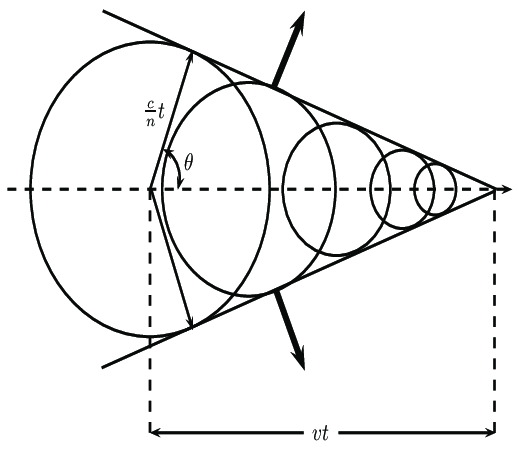
\includegraphics[scale=0.5]{Tesis-UNAM/Capitulo2/Figura-26-Representacion-pictorica-del-proceso-de-emision-de-radiacion-de-Cherenkov-La.png}
    \caption{Descripción bajo el esquema electrodinámico de la radiación Cherenkov}
    \label{fig:enter-label}
\end{figure}


El plano de el disco es perpendicular a la dirección del desplazamiento de la partícula, esta distribución es axisimétrica con respecto al vector de velocidad y simétrica con el plano medio del disco. Este campo eléctrico puede ser descrito como una superposición de ondas electromagnéticas planas, con estas consideraciones uno puede definir varios fotones virtuales con vectores de onda $\Vec{k}$ paralelos a $\Vec{v}$, y la componente transversal $\Vec{k}_\perp$ es cero\cite{Bashmakov_2015}.\\\\
Si la partícula se mueve a una velocidad mayor que la de la luz en el medio, el campo eléctrico en frente de la carga será nulo, la simetría axial se mantiene pero la distribución del campo eléctrico cambia a la de un cono. En la figura 2.2 se puede observar graficamente lo descrito anteriormente.\cite{Bashmakov_2015, Jelley}


\subsubsection{Mecanismos Físicos}
Debido al campo eléctrico generado por el movimiento de la partícula cargada, la distribución electrónica de las moléculas de la materia se verá afectada, causando que aparezcan diversos dipolos localizados en las inmediaciones de la partícula en movimiento\cite{Beyer, Jelley}. Cuando su velocidad es muy pequeña la distribución de estos dipolos es simétrica, pero al superar el umbral de la velocidad de la luz sobre el medio, debido al potencial retardado, la deformación de los orbitales electrónicos se vuelve asimétrica (fig 2.3), causando un campo dipolar resultante aun en puntos distantes de la carga. Cada uno de estos dipolos radiaran cómo una antena\cite{Beyer, Jelley}.\\

\begin{figure}[h!]
    \centering
    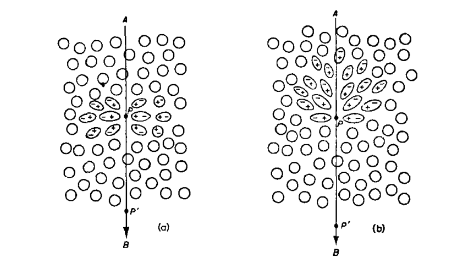
\includegraphics{Tesis-UNAM/Capitulo2/dipole.png}
    \caption{(a) Partícula con una velocidad baja (b) Partícula viajando a una velocidad mayor que la de la luz en el medio}
    \label{fig:enter-label}
\end{figure}

En un caso más realista el material tendrá un grosor considerable, esto implicará que los dipolos a lo largo de la trayectoria radien de forma sucesiva, aunque de tal forma que haya interferencia y que la emisión se propague en un ángulo fijo\cite{Jelley, Beyer}\\.

Usando esto como fundamento, Tamm y Frank pudieron mostrar\cite{Bashmakov_2015, Jelley, Beyer} que una partícula con carga Z que se mueve a una velocidad $v = \beta c$ en un medio con un indice de refracción $n\omega$ emitirá N fotones por cm recorrido en el medio en un intervalo de frecuencias $d\omega$

$$N(\omega)d\omega = \frac{2\pi Z^2 e^2}{\hbar c^2}\left(1 - \frac{1}{\beta^2n_\omega^2} \right)d\omega$$

Donde la emisión para una frecuencia específica se transmite en un ángulo Cerenkov determinado por la ecuación \cite{Bashmakov_2015, Jelley}

\begin{equation}
    cos\theta_\omega = \frac{1}{\beta n_\omega}
\end{equation}


\section{Detectores Cerenkov}

%Profundizar más, buscar bibliografía que te ayude
% Incluir efectos de dispersión y entender y explicar la física del proceso


\begin{figure}
    \centering
    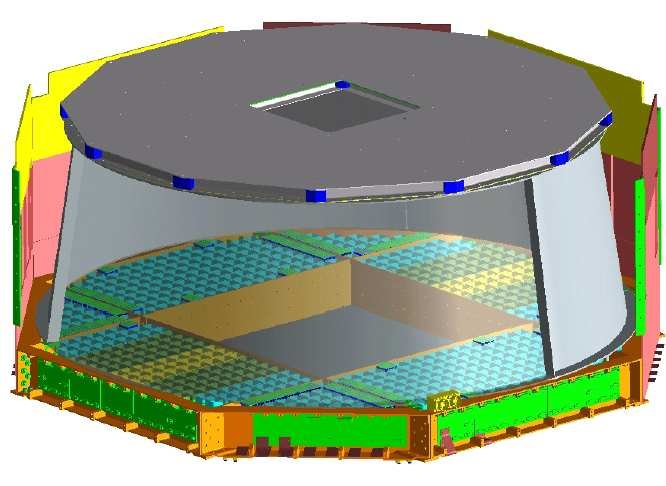
\includegraphics[scale=0.4]{Tesis-UNAM/Capitulo2/The-RICH-detector-of-AMS-02-left-View-of-the-assembled-RICH-detector-at-CIEMAT-right.jpg}
    \caption{Detector RICH de la misión AMS-02 \cite{AMSRICH}}
    \label{fig:enter-label}
\end{figure}

Una forma de estudiar el espectro y la composición de los rayos cósmicos es a través de la identificación de sus constituyentes y de la medición de su velocidad\cite{RICHCERN}, para esto es imprescindible el diseño de detectores con gran eficiencia. Esto es posible midiendo su masa y su carga eléctrica, a través de propiedades correlacionadas a la primera, cómo el momento la energía cinética y su velocidad $\beta$\cite{RICHCERN}, ya que si dos de ellas son medidas, se puede obtener la masa. En muchos experimentos, cómo es el caso de AMS-02, se acoplan varios detectores en conjunto, lo cuál permite cuantificar por separado las diferentes cantidades necesarias para la caracterización, e.g. la rigidez R midiendo el gyro radio de la partícula atravezando un campo magnético. Y a partir de la rigidez se obtiene el momento. Así que si consideramos un campo magnético B y el radiogiro de la partícula $\rho$

$$R = B\rho = \frac{p}{Z}$$
$$p = \gamma m_0c\beta$$
$$\Longrightarrow m_0 = \frac{RZ}{\gamma v}$$

Al obtener la masa en términos de la velocidad y el momento, uno puede ver la gran utilidad de los detectores cherenkov ya que este nos permite obtener la velocidad de la partícula, esto puede ilustrarse utilizando la ecuación (2.2) al obtener la relación entre el ángulo cherenkov y su masa.\cite{RICHCERN}

$$\frac{v}{c}=\beta=\frac{1}{n(\omega) cos\theta_\omega}$$
\begin{equation}
    \frac{RZn(\omega)}{c\gamma cos\theta}
\end{equation}

\subsection{Radiadores}
Los detectores Cerenkov son a grandes rasgos sensores de luz cerenkov emitida por partículas cargadas al atravesar un radiador, o sistema de radiadores. Estos radiadores pueden ser sólidos o gases\cite{RICHCERN}, tales que sean capaces de absorber o dispersar la menor cantidad de fotones posibles, y que dispongan con índices de refracción particulares dependiendo de la velocidad de las partículas que se pretenda caracterizar.\\

Por ejemplo, si queremos obtener $\beta$ en función del índice de refracción n, vemos el siguiente comportamiento (fig 2.4).\\

\begin{figure}[h!]
    \centering
    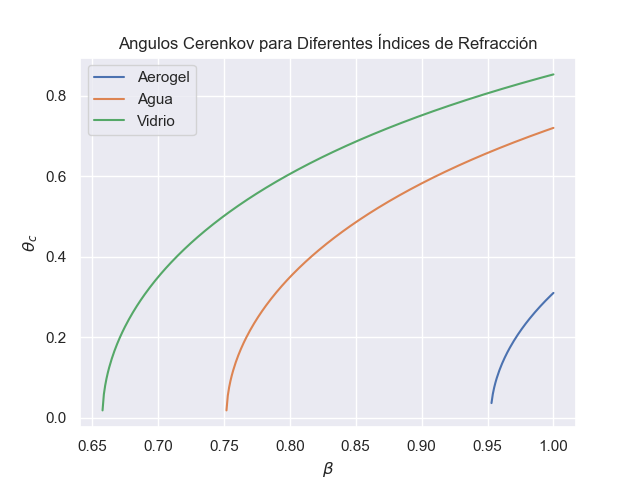
\includegraphics[scale=0.5]{Tesis-UNAM/Capitulo2/radiatorPrecision.png}
    \caption{Ángulo cerenkov contra beta}
    \label{fig:enter-label}
\end{figure}

Al incrementar la velocidad de la partícula, hasta el punto de llegar a la velocidad de la luz i.e. $\beta \longrightarrow 1$ se observa que $\theta = 1/n(\lambda)$, también se concluye que la sensibilidad es mayor al medir en angulos cerca de zonas donde $\frac{d\theta}{d\beta}$ es considerable, nótese que para protones (el cosntituyente más abundante de los rayos cósmicos) a una energía cerca de los 3-4 GeV, $\beta \approx 0.975$
el aerogel presenta una gran sensibilidad, en cambio para vidrio o agua el ángulo cerenkov empieza a saturarse más y más. Por esta razón es necesario utlizar el radiador adecuado en función de la velocidad estimada a medir por el radiador en cuestión.\\

Otras cuestiones de importancia serían que la luz cerenkov pueda atravesar el radiador con la menor perdida posible, debido a la poca cantidad de fotones emitidos por la partícula cargada en comparación a procesos centelladores, también hay que añadir que es muy importante que el radiador no centelleé de manera apreciable y además es crucial que el radiador sea transparante a la emisión cerenkov, que en la mayoría de los casos es en el rango del ultravioleta y que no haya bandas de absorción en el rango de operación\cite{RICHCERN}

\subsection{Sensores de Fotones}
El proposito fundamental de estos sensores es el de convertir la radiación cerenkov emitida por el radiador y convertirla en una señal eléctrica\cite{RICHCERN}, una consideración importante es que debido a la baja energía de los fotones cerenkov es que sólo es posible aprovechar cómo mecanismo de interacción de la luz con la materia la absorción fotoeléctrica, otra sería que el sensor debe de ostentar una eficiencia de detección alta de eléctrones individuales desprendidos de los átomos del material fotosensible.\\

Un tipo de  sensores con alta relevancia hoy en día serian los tubos PMT(Photomultiplier tubes) estos funcionan gracias al efecto fotoeléctrico. Aun que el experimento Helix tiene pensado implementar SiPM's (Silicon Photomultipliers) los cuales necesitan voltajes de polarización relativamente bajos y ostentan otra serie de ventajas e.g. un menor tamaño y peso.


%subsección
% Identificación de antinúcleos
% como se usa el RICH para identificar antinúcles a partír de la beta
% reconstrucción de masa y resolución de la masa (revisar presentaciones de ams)



\subsection{Experimentos Actuales}
En esta sección se presentará un breve recuento de los detectores RICH usados actualmante para remarcar la gran utilidad que poseen este tipo de experimentos para la física nuclear y de partículas.

\subsubsection{COMPASS} Detector RICH con radiador gaseoso de aceptancia ancha, donde se realizan detecciones de fotones únicos con detectores gaseosos y tubos fotmultiplicadores y haciendo uso de espejos esféricos. Ha conseguido la identificación de hadrones con un momento alto en el espectrometro COMPASS del CERN SPS, dedicado a estudiar la estructura hadrónica y a la espectroscopía hadrónica \cite{ALBRECHT2003112}

\subsubsection{Babar} La misión principal del experimento Babar es el estudio de las asimetrías que surgen en violaciones de la CP (paridad y carga) en el decaimiento de mesones neutrales B. Este experimento poseé el primer detector DIRC(Detector of Internally Reflected Cherenkov light), el cuál usa como radiador barras de cuarzo sumamente polidas. Se muestra un esquema de su funcionamiento.\cite{babas}

\begin{figure}[h!]
    \centering
    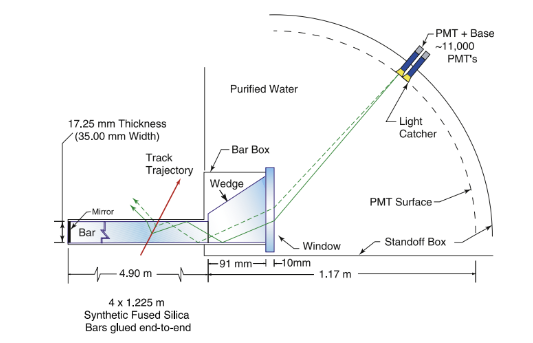
\includegraphics{Tesis-UNAM/Capitulo2/babasDirc.png}
    \caption{Caption}
    \label{DIRC del detector Babar}
\end{figure}

\subsubsection{LHCb} Una característica clave del diseño de este experimento es el de contar con dos RICH y tres tipos de radiadores aerogel, $C_4_{10}$ Y $CF_4$, el objetivo era identificar partículas con momento de 4-100 GeV/c. También cuenta con un novedoso detector de fotones, el HPD(Hybrid Pixel Detector), gracias a una considerable area sensible, se pudo obtener una buena cobertura geométrica a la vez de poder detectar una gran cantidad de fotones \cite{PAPANESTIS2020162004}

\pagebreak

\begin{figure}[h!]
    \centering
    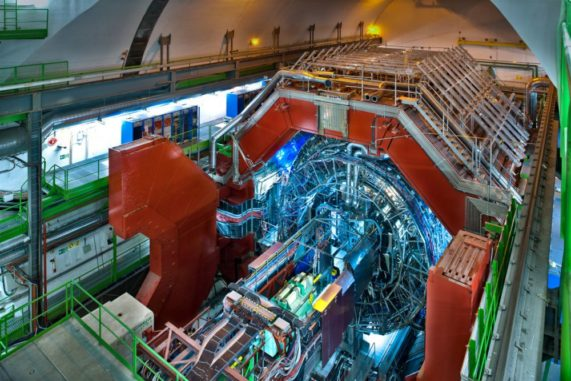
\includegraphics[scale=0.7]{Tesis-UNAM/Capitulo2/news_2765-571x381.jpg}
    \caption{Experimento ALICE}
    \label{fig:enter-label}
\end{figure}

\subsubsection{ALICE} El aparato ALICE consiste en estudiar colisiones $p^+p^+$, $p^+-Pb$ y $Pb-Pb$ proveidas por el LHC. Consiste de 7 Contadores RICH y usan $C_6F_{14}$ líquido cómo radiador, para detectar los fotones utiliza una cámara proporcional acoplada a un fotocatodo revestido de CsI \cite{VOLPE2014259}

\subsubsection{CBM} El experimento CBM está diseñado para estudiar las propiedades de la materia nuclear y mapear el diagrama de fase del QCD. E especial el RICH del CMB se planteo cómo una forma de detectar electrones con momento de hasta 8 GeV/c. Consiste de un radiador gaseoso de $CO_2$, un sistema de espejos esféricos, y de tubos fotomultiplicadores Hamamatsu \cite{ADAMCZEWSKIMUSCH201765}

\pagebreak

\subsubsection{AMS-02} 

%Profundizar en la descripción de AMS y otros experimentos de rayos cósmicos que tengan un RICH

El experimento AMS consta de un espectrómetro magnético de partículas de alta energía acoplado a la estación espacial internacional, lo que le brinda la gran ventaje de detectar rayos cósmicos sin haber interactuado con la atmósfera terreste. En el se encuentra un subdector RICH conformado de dos radiadores, uno de aerogel y otro de NaF, con tubos fotomultiplicadores. Ha sido el primer experimento en observar antinúcleos de helio. Para concluir el capítulo se tiene que enfatizar que este ha sido el detector utilizado cómo base de las simulaciones utilizadas para generar los datos a caracterizar.\cite{LIU20175}